%\documentclass{beamer}
\documentclass[RawSienna,dvipsnames]{beamer}

%%% Dichiarazione dei pacchetti standard.
\usepackage[italian]{babel}
\usepackage[utf8x]{inputenc}
%%% Personalizzazione del layout---articolata su cinque livelli.
%\usetheme{split}        % layout complessivo. 
\usetheme{CambridgeUS}
\useinnertheme{rectangles} % layout interno.
\useoutertheme{infolines} % layout esterno.
\setbeamercolor{title}{fg=RawSienna}
\setbeamercolor{frametitle}{fg=RawSienna}
\usecolortheme{crane} % schema di colori.
\usefonttheme{professionalfonts}  % schema dei font.
\setbeamercolor{item}{fg=RawSienna}
% Inutile dire che se volete tutti i default, potete risparmiarvi gli ultimi
% quattro comandi. 

%%% Titolo e autore.
\title{Monolith}
\subtitle{An interactive bubble provider}
\author{Revisione di Progettazione}
%\institute{Gruppo Utilizzatoti Italiani di \TeX}
%\date{\today}
\date{27 giugno 2017}

\begin{document}
	
\begin{frame}
	\begin{center}
		
\includegraphics[scale=0.13]{img/obelix.png}
		\qquad\qquad
		
\includegraphics[scale=0.13]{img/monolith.png}
	\end{center}
	\titlepage
\end{frame}


\section[Sommario]{}
\begin{frame}
	\tableofcontents
\end{frame}	

\section{Il gruppo Obelix}
\begin{frame}
	
	\begin{columns}
		\begin{column}{0.2\textwidth}
			
		\end{column}
		
		\begin{column}{0.4\textwidth}
			\begin{itemize}
				\item Emanuele Crespan
				\item Tomas Mali
				\item Silvio Meneguzzo
				\item Nicolò Rigato
				\item Riccardo Saggese
				\item Federica Schifano
			\end{itemize}
		\end{column}
		
		\begin{column}{0.2\textwidth}
			
		\end{column}
	\end{columns}


\end{frame}

\section{Introduzione}
\subsection{Cos'era una bolla?}
\begin{frame}
	\frametitle{Cos'era una bolla?}
	\begin{center}
		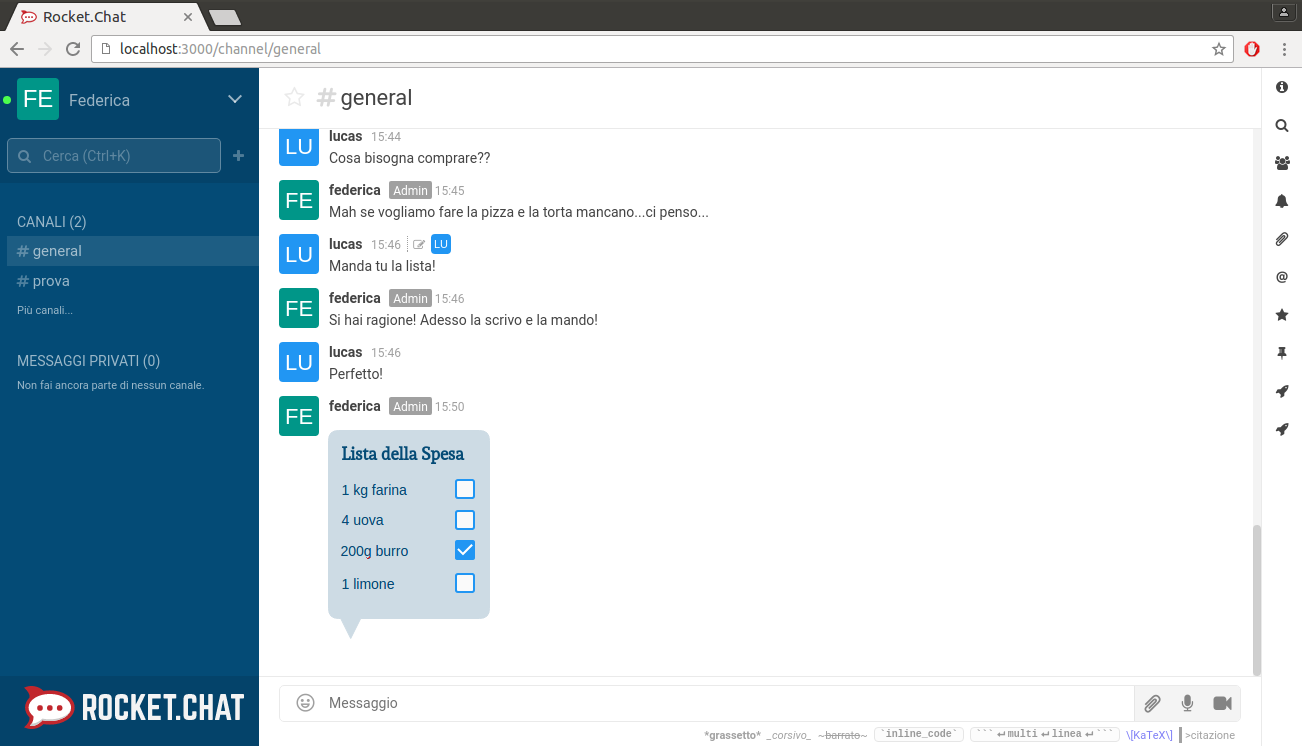
\includegraphics[scale=0.23]{img/f1.png}
	\end{center}
	
\end{frame}

\subsection{Cos'è una bolla?}
\begin{frame}
  \frametitle{Cos'è una bolla?}
  \textbf{Non più un messaggio speciale tra messaggi}
  \begin{center}
  	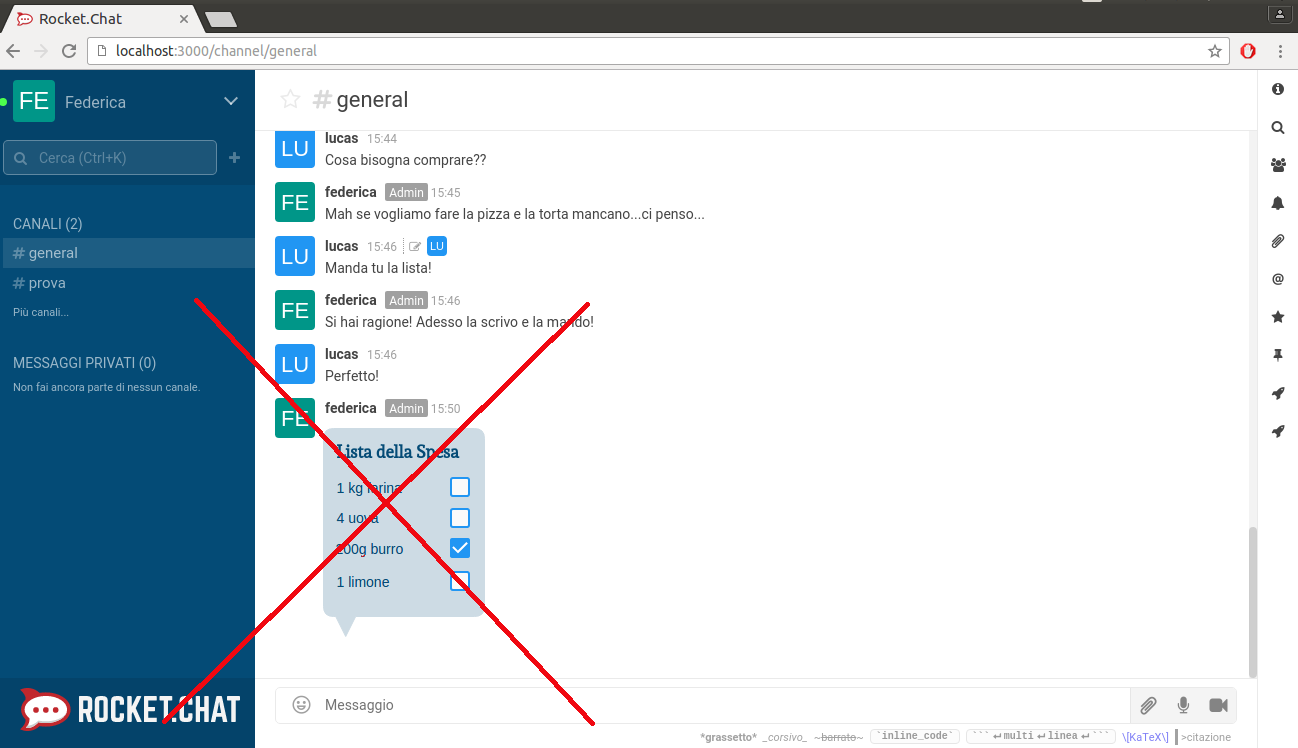
\includegraphics[scale=0.20]{img/f2.png}
  \end{center}

\end{frame}

%\subsection{prova3}
\begin{frame}
  \frametitle{Cos'è una bolla?}
% \framesubtitle{prova}
 \textbf{Un'applicazione eseguita in un'apposita SideArea}
\begin{center}
	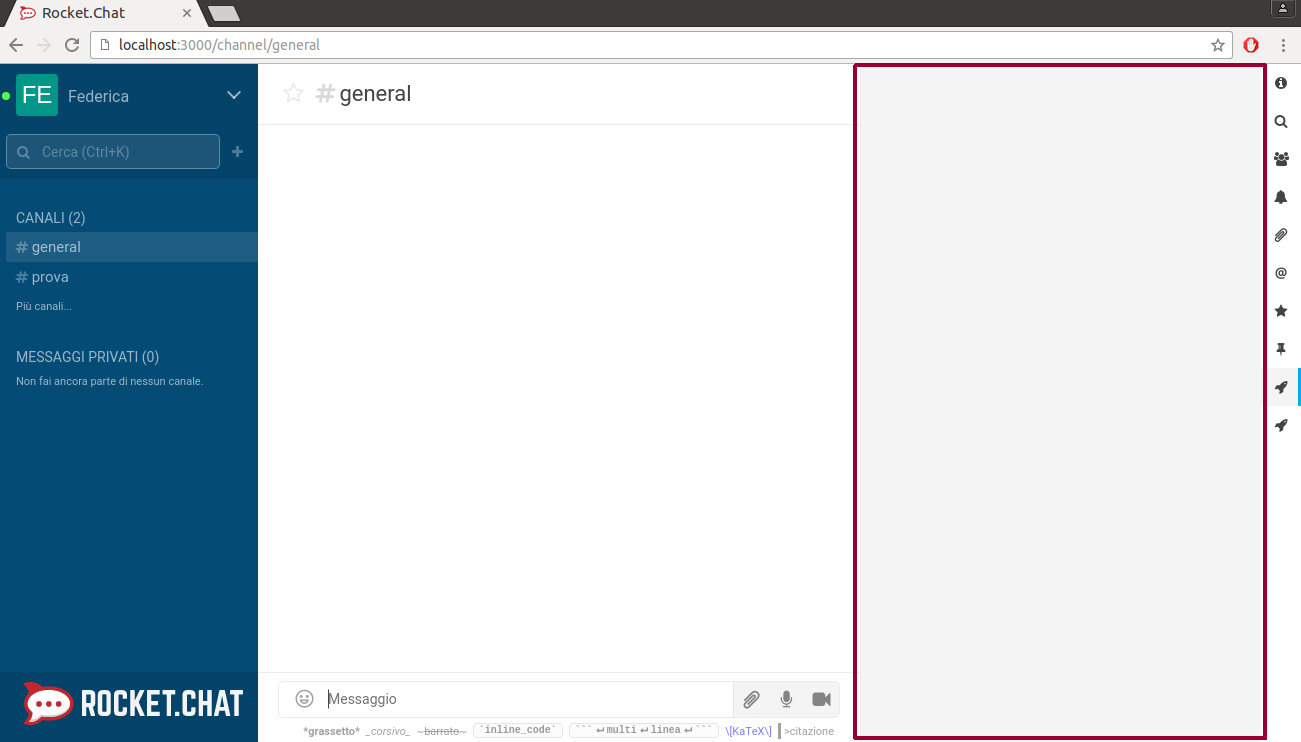
\includegraphics[scale=0.20]{img/f4.png}
\end{center}
 
\end{frame}

\begin{frame}
	\begin{figure}
		\begin{center}
			\caption{Due nuovi pulsanti nella tabbar laterale}
			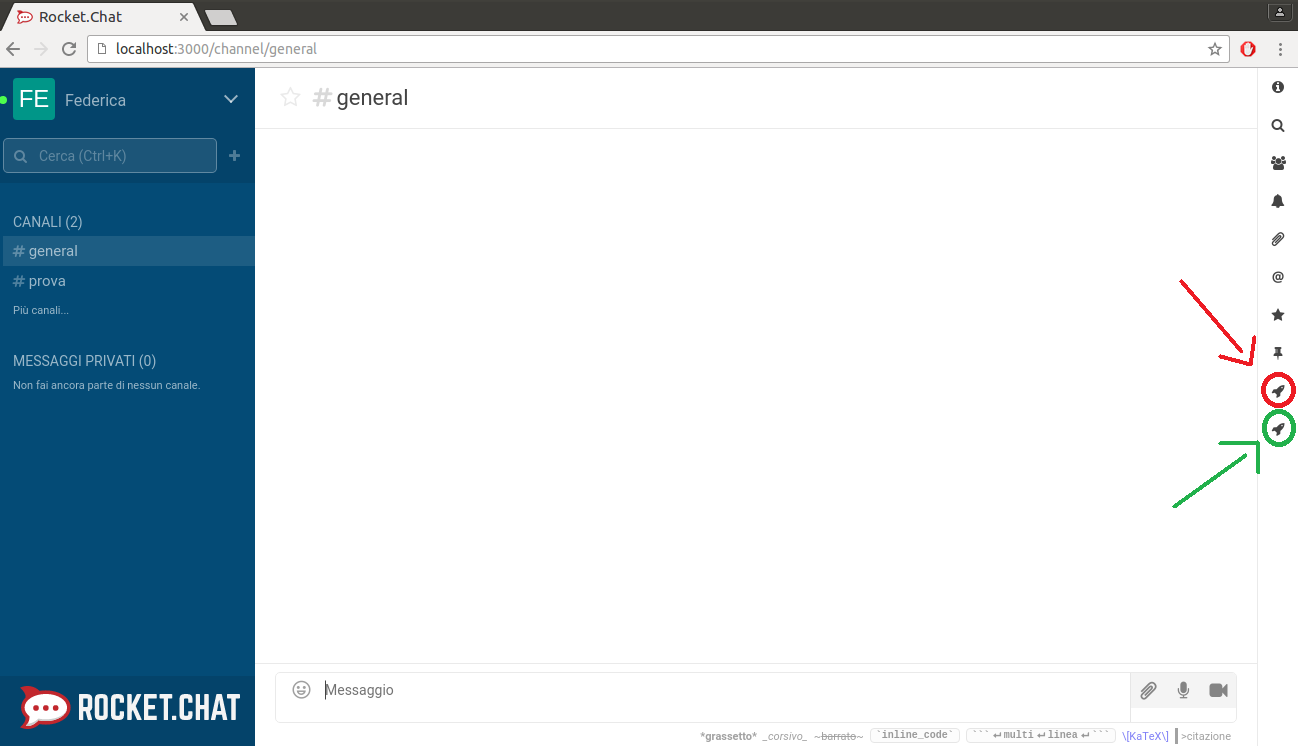
\includegraphics[scale=0.23]{img/f3.png}
		\end{center}
	\end{figure}	
\end{frame}

\begin{frame}
  
  \begin{center}
  	\begin{figure}
 		\caption{Storico delle bolle inviate e creazione di una nuova bolla}
  		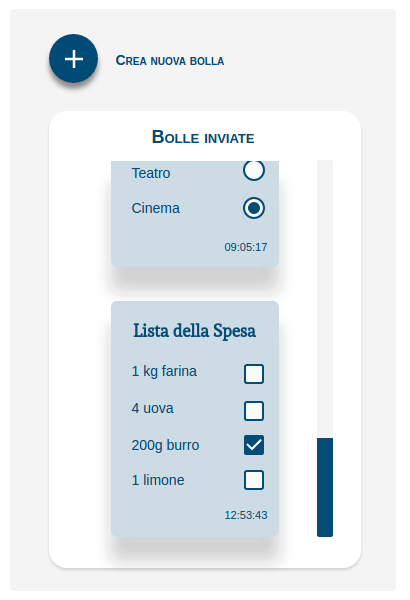
\includegraphics[scale=0.34]{img/mockup_1.png}
  	\end{figure}
  \end{center}
% \footnote{pie di pagina}
  
\end{frame}

\begin{frame}
	\begin{figure}
		\begin{center}
			\caption{Menù dei tipi di bolla}
			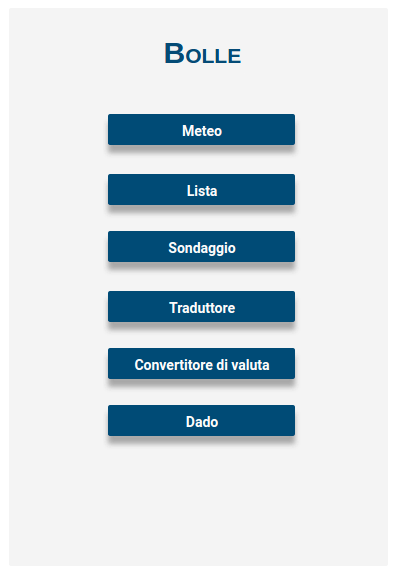
\includegraphics[scale=0.35]{img/mockup_2.png}
		\end{center}
	\end{figure}	
\end{frame}

\begin{frame}
	\begin{figure}
		\begin{center}
			\caption{Menù di configurazione di una bolla}
			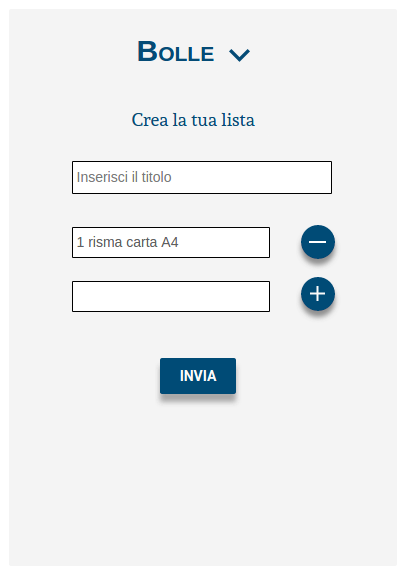
\includegraphics[scale=0.35]{img/mockup_3.png}
		\end{center}
	\end{figure}	
\end{frame}

\begin{frame}
	\begin{figure}
		\begin{center}
			\caption{Due nuovi pulsanti nella tabbar laterale}
			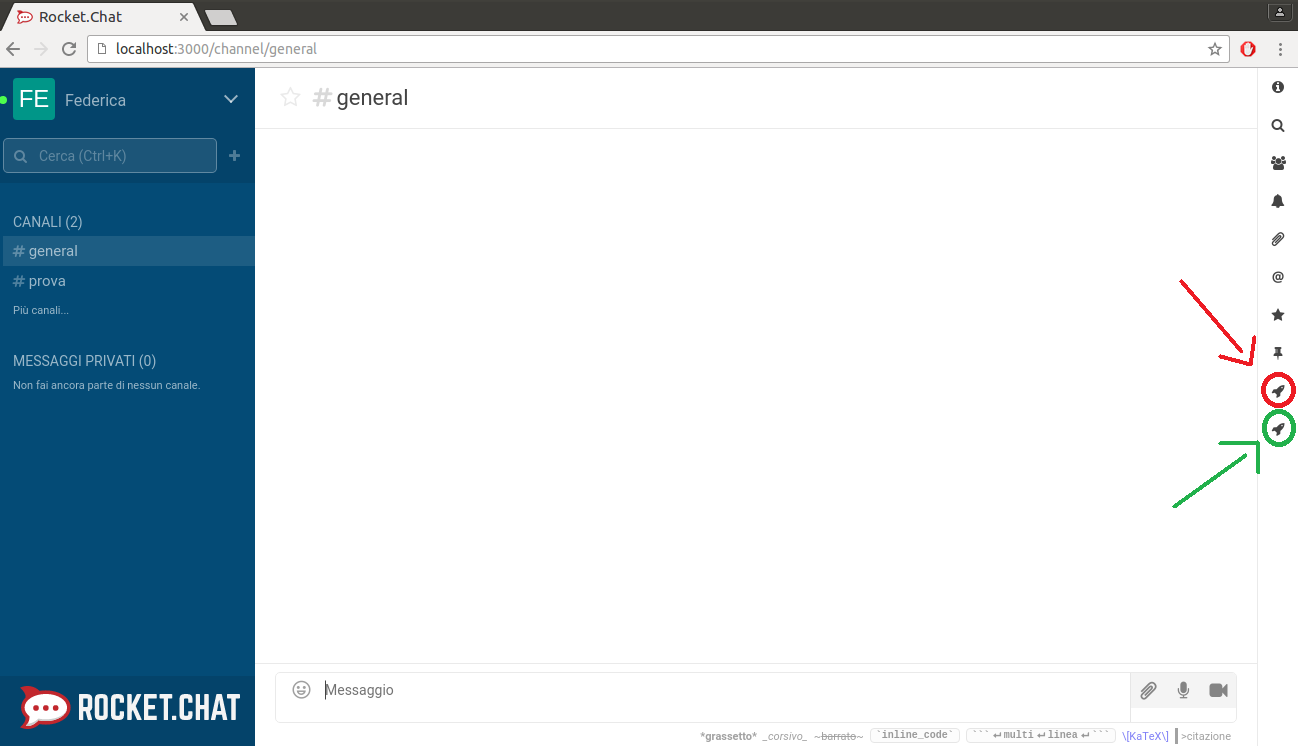
\includegraphics[scale=0.23]{img/f3.png}
		\end{center}
	\end{figure}	
\end{frame}

\begin{frame}
	\begin{figure}
		\begin{center}
			\caption{Storico delle bolle ricevute}
			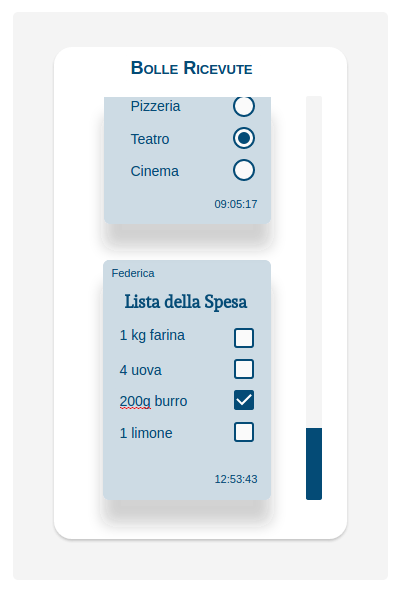
\includegraphics[scale=0.35]{img/mockup_4.png}
		\end{center}
	\end{figure}	
\end{frame}

\begin{frame}
\frametitle{Vantaggi}	
	\begin{columns}
		\begin{column}{0.2\textwidth}
			
		\end{column}
		
		\begin{column}{0.4\textwidth}
		%	\textbf{Vantaggi}:
			\begin{itemize}
				\item Bolle indipendenti dai messaggi
				\item Configurazione della bolla in spazio adeguato
				\item Interfaccia responsive
			\end{itemize}
		\end{column}
		
		\begin{column}{0.2\textwidth}
			
		\end{column}
	\end{columns}
	
\end{frame}
 %fede

\section{Descrizione prodotto}


\subsection{Monolith SDK}


\begin{frame}
  \frametitle{Funzionamento SDK}
  \begin{center}
    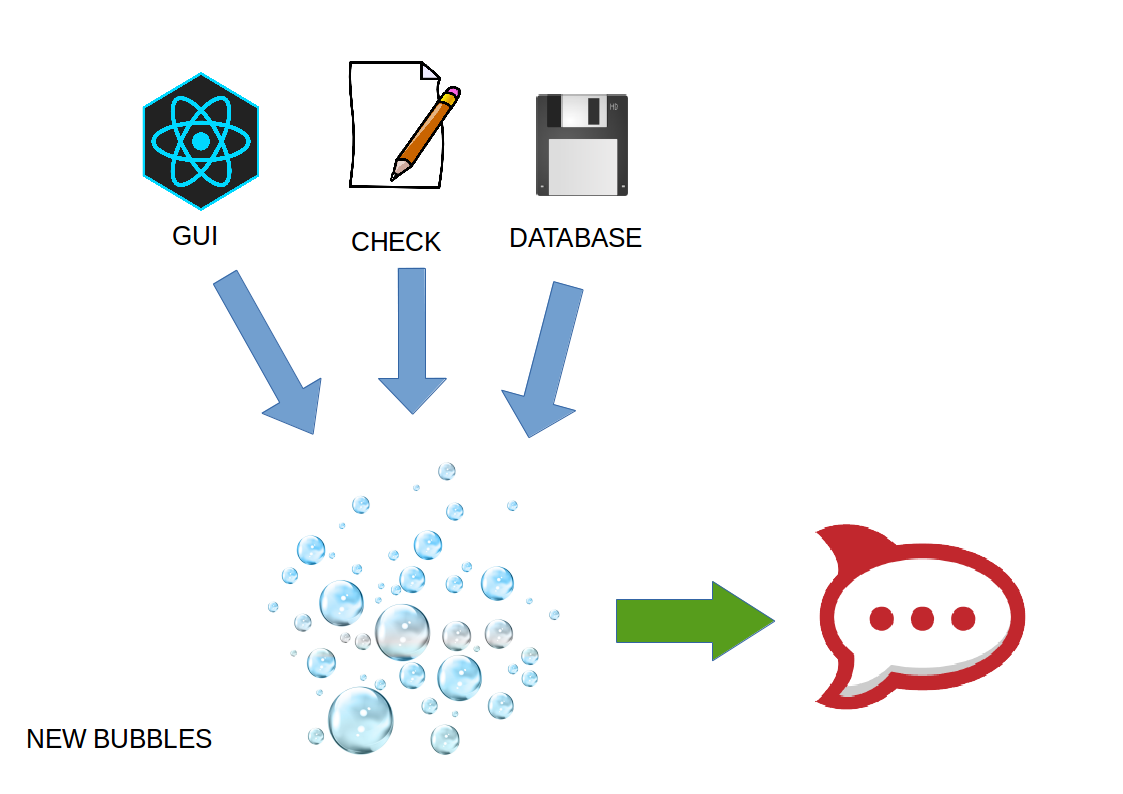
\includegraphics[width=\linewidth,height=.8\textheight,keepaspectratio]{img/uso_sdk.png}
  \end{center}
\end{frame}

\begin{frame}
  \begin{columns}[T] % align columns
    \begin{column}{.48\textwidth}
      \textbf{Creazione GUI}
      \begin{itemize}
      \item Bubble
        \begin{itemize}
        \item Sender
        \item Receiver
        \end{itemize}
        \pause
      \item Configuration Menu
      \item Button
        \begin{itemize}\pause
        \item[$ \rightarrow $] Personalizzazione
        \end{itemize}
      \end{itemize}
    \end{column}
    \pause
    \begin{column}{.48\textwidth}
      \textbf{Server Side Operations}
      \begin{itemize}
      \item[] Meteor.method
        \begin{itemize}
        \item insert  $ \rightarrow $ Custom method
        \item update $ \rightarrow $ Custom method
        \item remove
        \end{itemize}
      \end{itemize}
    \end{column}

  \end{columns}

\end{frame}
 %nicolò e tomas

\subsection{Interfaccia}
\begin{frame}
	\frametitle{Interfaccia}
	\begin{center}
	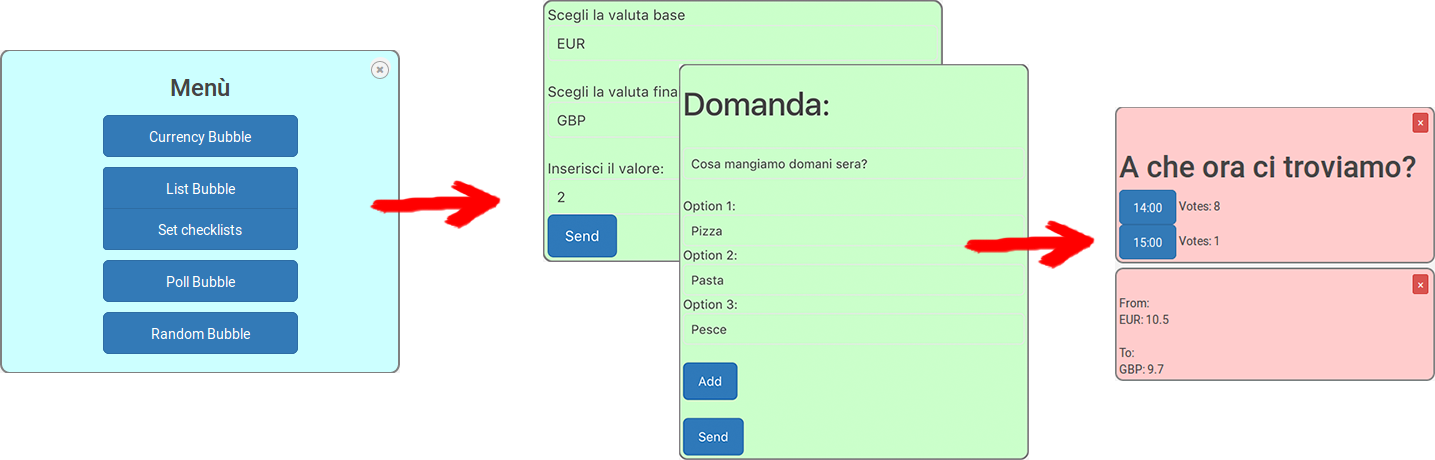
\includegraphics[scale=0.22]{img/interf.png}
	\end{center}
\end{frame}


\begin{frame}
	\frametitle{CSS}
	\begin{center}
	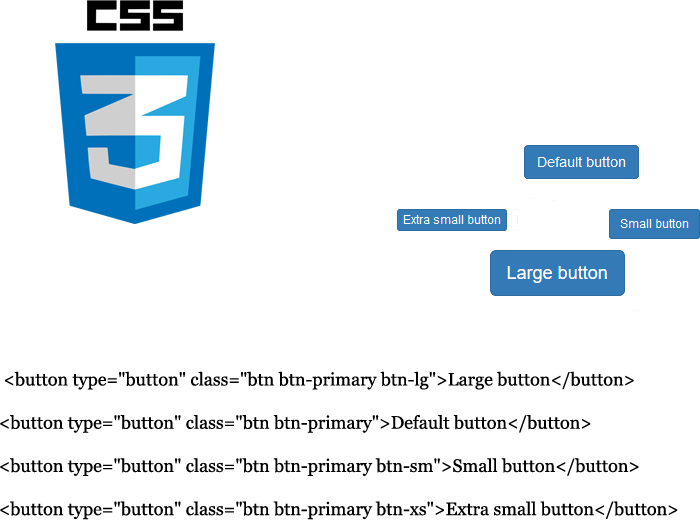
\includegraphics[scale=0.35]{img/css.png}
	\end{center}
\end{frame}

\subsection{Demo}
\begin{frame}
	\frametitle{Demo: lista}
	\begin{center}
	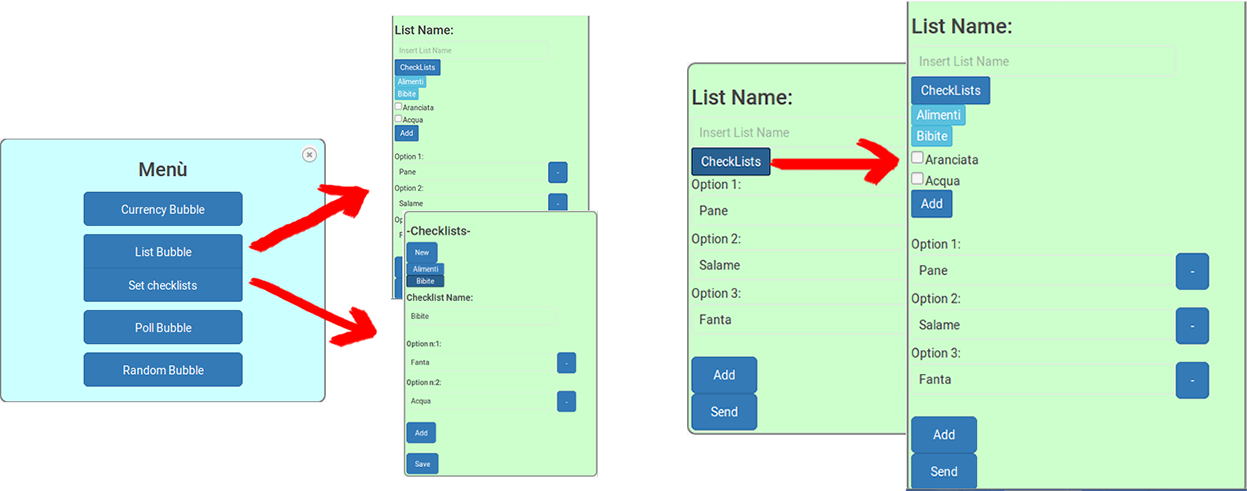
\includegraphics[scale=0.25]{img/demo.png}
	\end{center}
\end{frame}
 %emanuele

\section{Modifiche Apportate}
\subsection{Generali}

\begin{frame}
	\frametitle{Modifiche Generali}
	
		
		\begin{columns}
			\begin{column}{0.2\textwidth}
				
			\end{column}
			
			\begin{column}{0.4\textwidth}
				\begin{itemize}
					\item Numero di versione per documento
					\item Registro delle modifiche
					\item Verbali
				
				\end{itemize}
			\end{column}
			
			\begin{column}{0.2\textwidth}
				
			\end{column}
		\end{columns}
		
		
\end{frame}


\subsection{Documenti}

\begin{frame}
	\frametitle{Modifiche Documenti}
	
	
	\begin{columns}
		\begin{column}{0.2\textwidth}
			
		\end{column}
		
		\begin{column}{0.4\textwidth}
			\begin{itemize}
				\item Norme di Progetto
				\item Analisi dei Requisiti
				\item Piano di Progetto
				\item Piano di Qualifica
				
			\end{itemize}
		\end{column}
		
		\begin{column}{0.2\textwidth}
			
		\end{column}
	\end{columns}
	
\end{frame} %silvio

\section{Consuntivo e Preventivo a finire}
%\subsection{Progettazione Architetturale}
\begin{frame}
  \frametitle{Consuntivo}
  \begin{center}
  	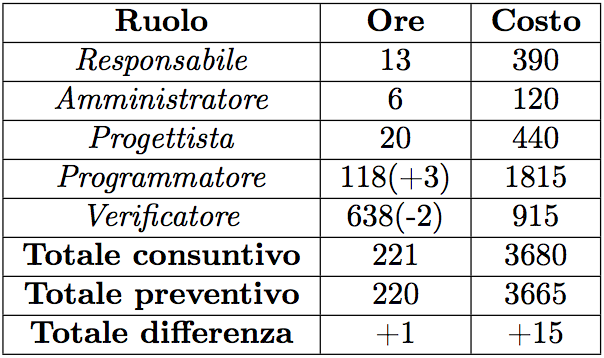
\includegraphics[scale=0.5]{img/prevCD}
  	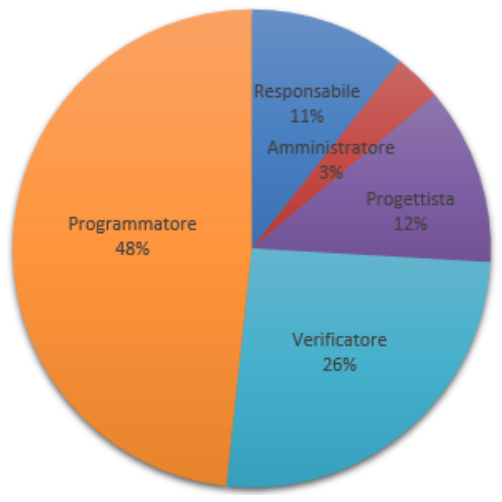
\includegraphics[scale=0.4]{img/cakeCD}
  \end{center}
%Rispetto al preventivo, sono emerse differenze con una diminuzione di 2 ore per il ruolo di Verificatore ed una maggiorazione di 3 ore per quello del Programmatore.
\end{frame}

\begin{frame}
	\frametitle{Preventivo a finire}
	
	\begin{center}
		\centering
		\begin{tabular}{|c|c|}
			\hline
			\textbf{Periodo} & \textbf{Diff} \\
			\hline
			\emph{Analisi dei requisiti}  & 0 \\
			\hline  \emph{Analisi in Dettaglio}  & -15 \\
			\hline  \emph{Progettazione Architetturale}  & +31 \\
			\hline  \emph{Progettazione in Dettaglio}  & +58 \\
			\hline  \emph{Codifica}  & +15 \\
			\hline  \emph{\textbf{Totale}}  & +89 \\
			\hline
		\end{tabular}
	\end{center}
	
Tenendo conto del risultato dei consuntivi nei periodi precedenti, il bilancio totale risulta negativo per 89 \euro.\\

\end{frame}

 %riccardo

\end{document}
